\documentclass{ximera}

\input{preamble.tex}

\author{Gregory Hartman \and Matthew Carr}
\license{Creative Commons 3.0 By-NC}
\acknowledgement{https://github.com/APEXCalculus}

\begin{document}


\begin{exercise}

\outcome{Evaluate the limit as $x$ approaches a point where there is a vertical asymptote.}
\outcome{Identify when a limit does not exist.}

\tag{limit} 
\tag{discontinuous}
\tag{vertical asymptote}

  Find 
  \[
  \displaystyle \lim_{x\to0} \frac{x+1}{x^2+3x}
  \begin{prompt}
  = \answer{\text{Limit does not exist}}.
  \end{prompt}
  \]
    \begin{hint}
      This function is \underline{not} continuous everywhere, but both the numerator and denominator are continuous everywhere as functions. Thus, if the limit of $\frac{x+1}{x^2+3x}$ as $x\to a$ does not exist, then the denominator $x^2+3x$ must be zero at $a$.
    \end{hint}
     \begin{hint}
    Take a look at the graph of the function
    \begin{center}
     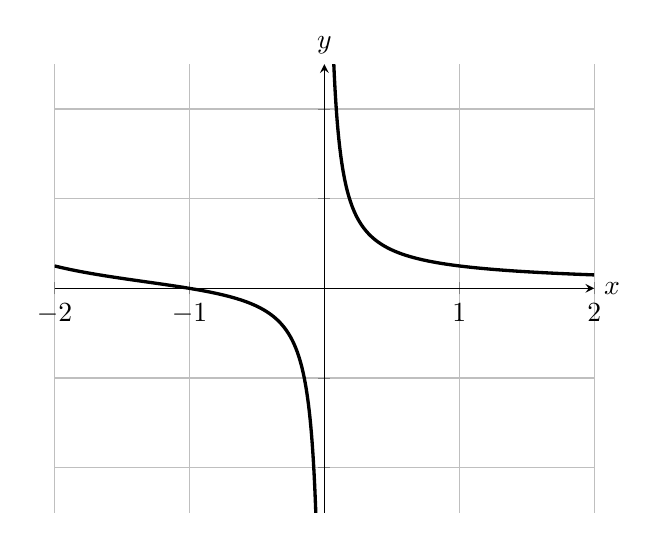
\begin{tikzpicture}
	\begin{axis}
	[ymin=-5,ymax=5, axis lines=center,xlabel=$x$,ylabel=$y$,every axis y 
	label/.style={at=(current axis.above origin),anchor=south},every axis x label/.style={at=(current axis.right of origin),anchor=west},
	domain=-2:2,
	yticklabels={},
	ymajorgrids=true,
	grid = major
	]
	\addplot[domain=-2:-1/100,very thick,smooth,samples=500]
	{(\x+1)/(\x^2+3*\x)};
	\addplot[domain=1/100:2,very thick,smooth,samples=500]
	{(\x+1)/(\x^2+3*\x)};
	\end{axis}
       \end{tikzpicture}      
      \end{center}
     Apply the limit law that $\lim\limits_{x\to{a}}\frac{f(x)}{g(x)}=\frac{\lim\limits_{x\to a}f(x)}{\lim\limits_{x\to{a}}g(x)}$ if $g(a)\ne0$ and both $f(x)$ and $g(x)$ are continuous at $x=a$. Observe what happens around $x=0$.
    \end{hint}
    \begin{hint}
     On the one hand, $-3< x<0$, $x^2+3x<0$ and for $-1<x<0$, $x+1>0$; hence, for $-1<x<0$, $\frac{x+1}{x^2+3x}<0$. On the other hand, for every number $a$ satisfying $-1<a<0$, the limit  $\lim\limits_{x\to a}\frac{x+1}{x^2+3x}$ exists because both functions are continuous between $-1$ and $0$, noninclusive. Applying several limit laws tells us that $\lim\limits_{x\to a}x+1=\left(\lim\limits_{x\to a}x\right)+\left(\lim\limits_{x\to a}1\right)=a+1$ and $\lim\limits_{x\to a}x^2+3x=\left(\lim\limits_{x\to a}x\right)^2+3\cdot\left(\lim\limits_{x\to a}x\right)=a^2+3a$. Hence, $\lim\limits_{x\to a}\frac{x+1}{x^2+3x}=\frac{a+1}{a^2+3a}$.
     
     Combining these two observations with the fact that the denominator becomes arbitrarily close to $0$ as $a$ approaches $0$, while the numerator approaches $1$, we see that $\lim\limits_{x\to0^{-}}\frac{x+1}{x^2+3x}$ is negative, but does not approach any finite number. We do not say that $-\infty$ is a valid limit, so the limit does not exist, regardless of whether or not the limit as $x\to0^{+}$ tends towards $-\infty$ as well.
     \end{hint}
\end{exercise}

\end{document}